% RA-L submission version. Full-length draft (arXiv / long version): paper_long.tex
\documentclass[letterpaper, 10pt, journal, twoside]{IEEEtran}

\usepackage{cite}
\usepackage{amsmath,amssymb}
\usepackage{booktabs}
\usepackage{graphicx}
\usepackage{xcolor}
\usepackage{url}
\usepackage{hyperref}

\graphicspath{{figures/}}

% Convenience macro for TODO markers left in the manuscript during drafting.
\newcommand{\todo}[1]{\textcolor{red}{\textbf{[TODO:} #1\textbf{]}}}

\title{Grasp-Taxonomy Conditioning as a Mode Switch\\for Dexterous Grasping of Climbing Holds}
\author{Anonymous Authors}

\markboth{IEEE Robotics and Automation Letters. Preprint Version.}%
{Grasp-Taxonomy Conditioning as a Mode Switch}

\begin{document}
\maketitle

\begin{abstract}
Dexterous grasping in robotics relies on distinct hand configurations depending on
object geometry. In our testbed of rock climbing holds this becomes evident in styles
of holds, for thin edges a crimp is required, for slopers an open hand press is
required, etc. Existing diffusion-policy approaches learn the singular action
distribution per task, but don't model grasp taxonomy. This leaves the question of how
taxonomy conditioning will impact the learned distribution. We introduce
\textbf{BetaGrasp}, a grasp-taxonomy-conditioned 3D diffusion policy that builds off a
DP3-style point-cloud policy on a four-class label (crimp, sloper, pinch, and jug) for
a Franka arm with a 16-DoF LEAP hand end effector. In climbing, ``beta'' is the
knowledge of how to do a move, which climbers often get from someone else rather than
from looking at the hold. The grasp-type label plays the same role for our policy.
This is done in conjunction with a
climbing-hold manipulation benchmark on a spring-constrained displacement testbed with
a linear ratchet that produces a slip-force readout in newtons. With climbing holds this matters,
because the point clouds of different holds look alike to the policy's encoder, so the
scan alone can't tell it which grasp to use. The trained models we
evaluated showed that the system without grasp-taxonomy does have classical
mode collapse once it starts from the robot's reset pose: in closed-loop rollouts it
ends in a jug grasp on every hold (25\% correct grasp type, versus 94\% with
taxonomy). In other words, the taxonomy label acts as a switch for which grasp the
policy performs. Hardware
evaluation on 80 paired trials supports this
mechanistic prediction. Taxonomy conditioning improves median slip force by +5.2\,N
(Wilcoxon signed-rank, $p < 0.001$, Cohen's $d = 0.95$), with the smallest effect on
the jug ($d = 0.55$), the grasp the system without taxonomy defaults to, and the
largest on pinch ($d = 1.82$). The
system's failure mode was grasps slipping on holds; this drops from 44\% of trials
without grasp taxonomy to 10\% with grasp taxonomy.
\end{abstract}

\begin{IEEEkeywords}
Dexterous manipulation, imitation learning, deep learning in grasping and manipulation,
grasping.
\end{IEEEkeywords}

% -----------------------------------------------------------------------
\section{Introduction}
% -----------------------------------------------------------------------

\begin{figure*}[t]
\centering
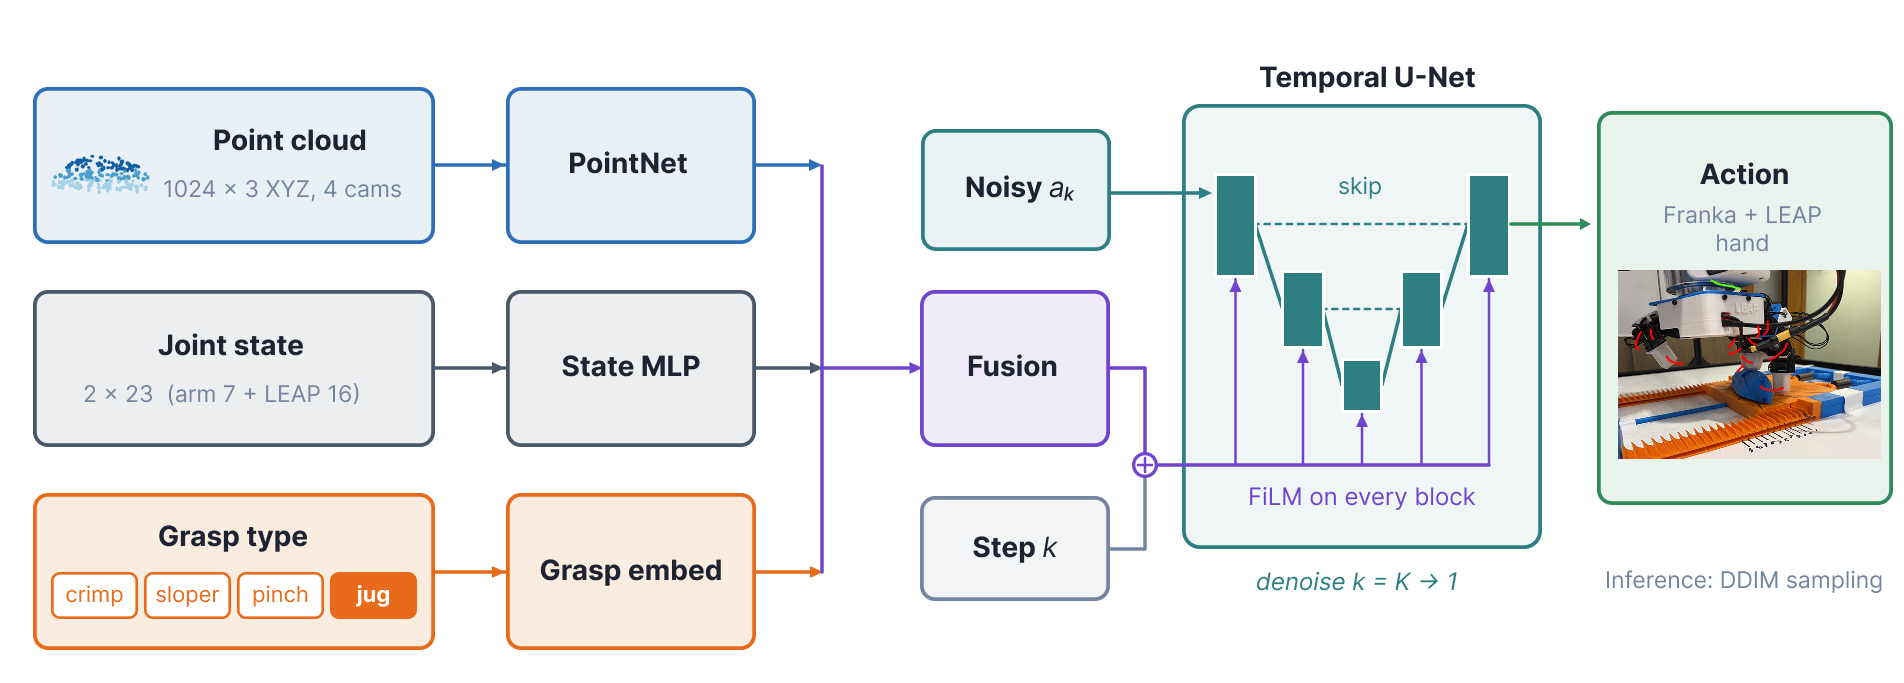
\includegraphics[width=\textwidth]{fig_architecture.png}
\caption{BetaGrasp architecture. Point cloud, proprioception, and grasp-type
label are encoded independently and fused into a 512-d conditioning vector $z$
that feature-wise conditions a 1D temporal U-Net diffusion denoiser. The
without-taxonomy ablation drops only the grasp-type branch (orange)
(37{,}248 parameters, $0.1\%$ of 34.6\,M).}
\label{fig:arch}
\end{figure*}

\IEEEPARstart{I}{mitation} learning based manipulation has developed rapidly on
parallel-jaw claw grippers. Development on multi-finger end effectors has been slower
to follow, because the subtle changes in object geometry require equally subtle changes
in hand finger formations. Within the domain of climbing holds the way and grip created
to grasp onto a hold directly determines how much force a grip can exert before
slipping off. In this paper we split the same high level task (``grasp the hold'') into
4 distinct strategies: \emph{crimp} (tight curled fingertips on thin edges),
\emph{sloper} (open-hand full contact frictional pressing), \emph{pinch} (thumb-ulnar
finger opposition), and \emph{jug} (ulnar digits grasp incut handles). Each of these
grasp strategies correspond to different feasible hand positions and contact spaces,
with different failure modes under load.

Diffusion-based behavior cloning has become the standard for visuomotor policy
learning \cite{chi2023diffusionpolicy,ho2020ddpm}. We built on top of DP3
\cite{ze2024dp3}, a 3D diffusion policy that operates on point clouds, as our base
architecture (Fig.~\ref{fig:arch}). The problem arises for multi-grasp policies in how
grasping distribution is mapped out. Most diffusion policies treat grasping as a single
distribution conditioned on observations. These observations from point-clouds alone
lack explicit conditioning on grasp taxonomy. This is especially a problem for climbing
holds. Once the scene is cropped and downsampled to 1024 points, the policy's encoder
can't tell the four holds apart, even though each one needs a different grasp. Recent work on taxonomy-conditioned
grasping \cite{dexonomy2025,tian2024graspasyousay} does train on grasp type but only
generates static poses on an end effector, rather than executable autonomy
trajectories, leaving execution-policy open.

The natural hypothesis is that taxonomy conditioning helps as a \emph{mode selector}.
Without taxonomy a policy trained on multi grasp datasets could collapse to one grasp
type and fail when faced with a mixed test set. In our example, it could collapse to,
say, a jug grasp every time and fail for the other 3 grasping tasks. Our analysis
supports this theory. Started from the robot's reset pose, the without-taxonomy policy
collapses to a jug grasp on every hold. It only separates grasp types when its starting
hand pose already carries them, as in the first frame of a recorded demonstration. This
prediction is testable on hardware: conditioning should help least on the jug, the
grasp the without-taxonomy policy defaults to. The
empirical per-type success pattern follows suit. Like a climber who has been given the
beta, the policy with the taxonomy label knows which grasp to use before it reaches the
hold; without it, the policy has to guess from a point cloud that doesn't distinguish
the holds.

\paragraph*{Contributions}
\begin{enumerate}
  \item A \textbf{grasp-taxonomy-aware 3D diffusion policy} (BetaGrasp) that
    conditions action diffusion on a grasp-type label alongside 3D point-cloud
    geometry and robot proprioception, built on DP3-style architectures
    \cite{ze2024dp3}.
  \item A \textbf{climbing-hold manipulation benchmark}, where the holds look alike to
    the policy as point clouds but each need a different grasp, with a
    spring-constrained displacement testbed and linear ratcheting mechanism, providing continuous
    grip-stability measurements across five hold orientations per grasp/hold type.
  \item A \textbf{mechanistic characterization} showing that taxonomy conditioning
    acts as a mode selector at deployment (without it, the policy collapses to a jug
    grasp from the reset pose, because the point cloud alone does not identify the
    grasp), with evidence from latent-space
    analysis, closed-loop rollouts, and per-type robot evaluation.
  \item A \textbf{paired evaluation protocol} with global model-order
    alternation and per-trial point-cloud capture, supporting Wilcoxon signed-rank
    inference and Cohen's $d$ on paired differences.
\end{enumerate}

% -----------------------------------------------------------------------
\section{Related Work}
% -----------------------------------------------------------------------
\subsection{Diffusion Policies for Robot Control}
Diffusion Policy \cite{chi2023diffusionpolicy} formulates behavior cloning as
conditional denoising. It's responsible for generating action trajectories via a
temporal U-Net that is conditioned on observations. This approach uses the
multimodality of diffusion models \cite{ho2020ddpm} and often accelerates inference
with DDIM \cite{song2021ddim}.

DP3 \cite{ze2024dp3} builds on diffusion policy to extend its tooling to point-cloud
observation inputs using a PointNet-style encoder \cite{qi2017pointnet}. The subsequent
work extends this to larger backbones and broader task families \cite{ze2024idp3}.
Category-level generalization using 3D semantic fields has achieved substantial gains
on unseen instances \cite{wang2024gendp}. Diffusion models have also been applied to
grasp synthesis and dexterous grasp generation \cite{weng2024dexdiffuser}.

\subsection{Dexterous Manipulation Data and Embodiments}
DexCap \cite{wang2024dexcap} proposes scalable mocap-based pipelines for hand--arm
systems, providing practical guidance on sensors, calibration, and capture rates. For
teleoperation we build directly on the open-source OpenVR codebase
\cite{george2023openvr}, a VR-based system for the Franka arm originally paired with an
Allegro hand. Our modifications retarget the hand interface from the Allegro to the
LEAP Hand v1, which provides the wider finger range of motion required for our
four-class taxonomy. Functional pre-grasp manipulation has been studied via diffusion
policy with teacher-student distillation \cite{wu2024unidexfpm}. CrossDex
\cite{crossdex2025} addresses cross-embodiment generalization via eigengrasp
representations. Our work is complementary, targeting qualitatively distinct grasps
on a fixed embodiment.

\subsection{Grasp Taxonomy and Type-Conditioned Grasping}
Human grasp taxonomies organize grasps into discrete categories reflecting opposition
type, thumb position, and power vs.\ precision \cite{feix2016grasp}.
Most closely related, \textbf{Dexonomy} \cite{dexonomy2025} conditions on the full
33-type GRASP taxonomy from single-view point clouds to synthesize dexterous grasp
poses for a Shadow Hand (82.3\% real-world success). Dexonomy is a static
grasp-pose generator: it produces three snapshots (pre-grasp, grasp, squeeze) handed to
a motion planner, with no imitation learning and no continuous trajectory execution.
Language-conditioned grasp generation \cite{tian2024graspasyousay} similarly produces
static poses. OmniDexVLG \cite{omnidexvlg2024} uses a VLM to infer taxonomy type,
feeding a downstream pose generator. DexGraspVLA \cite{dexgraspvla2026} combines a VLM
planner with a diffusion execution policy, but the VLM selects \emph{which object} to
grasp rather than \emph{how}; no per-type trajectory specialization is learned.

To our knowledge, BetaGrasp is the first system to condition a continuous
imitation-learning execution policy on grasp taxonomy for a multi-DoF arm--hand system,
and the first to show what that conditioning changes in the policy's behavior. Table~\ref{tab:novelty} summarizes the positioning.

\begin{table}[t]
\centering\small
\setlength{\tabcolsep}{3pt}
\caption{Positioning along four axes: point cloud input, grasp-taxonomy
conditioning, continuous execution policy (vs.\ static pose generation), and
dexterous hand.}
\label{tab:novelty}
\begin{tabular}{lcccc}
\toprule
Method & PC & Taxonomy & Exec.\ policy & Dex.\ hand \\
\midrule
DP3 \cite{ze2024dp3}                          & \checkmark & ---        & \checkmark   & Allegro \\
Dexonomy \cite{dexonomy2025}                  & \checkmark & 31 types   & pose-gen     & Shadow \\
Grasp as You Say \cite{tian2024graspasyousay} & \checkmark & language   & pose-gen     & \checkmark \\
OmniDexVLG \cite{omnidexvlg2024}              & partial    & VLM        & pose-gen     & \checkmark \\
DexGraspVLA \cite{dexgraspvla2026}            & ---        & obj.\ ID   & \checkmark   & \checkmark \\
\textbf{BetaGrasp}                            & \checkmark & 4-class    & arm+hand     & LEAP \\
\bottomrule
\end{tabular}
\end{table}

% -----------------------------------------------------------------------
\section{Method: Grasp-Taxonomy-Aware 3D Diffusion Policy}
\label{sec:method}
% -----------------------------------------------------------------------

\subsection{Problem Formulation}
We consider episodic manipulation of a static climbing hold on a tabletop workspace.
At each control step $t$, the policy observes (i) a fused point cloud
$P \in \mathbb{R}^{N \times 3}$ (captured once per episode after parking the arm out
of the cameras' field of view), (ii) a proprioceptive state history $s_{t-T_o+1:t}$
over observation horizon $T_o$, and (iii) a grasp-type label $g \in \{0,1,2,3\}$
corresponding to \{crimp, sloper, pinch, jug\}. The policy outputs a joint-space
action chunk $a_{t:t+T_p-1}$ over prediction horizon $T_p$; the controller executes
the first $T_a \le T_p$ steps before replanning. The label $g$ is provided manually
during data collection and at deployment time.

Following Chi et al.~\cite{chi2023diffusionpolicy}, we model the conditional
distribution over action sequences as a denoising diffusion process,
$p(a_{t:t+T_p-1} \mid P, s_{t-T_o+1:t}, g)$, learned from teleoperated demonstrations
via supervised diffusion loss.

\subsection{Architecture}
\label{sec:arch}
Our policy follows the DP3 design pattern \cite{ze2024dp3}: a point-cloud encoder
produces a 3D scene embedding, fused with robot state and a grasp-type embedding to
condition a 1D temporal U-Net that parameterizes the diffusion denoiser
(Fig.~\ref{fig:arch}).

\paragraph*{Point cloud encoder}
A PointNet-style encoder \cite{qi2017pointnet} (channels $3 \to 64 \to 128 \to 256$,
no T-Net, max-pool, linear projection) maps $P \in \mathbb{R}^{1024 \times 3}$ to a
256-dimensional feature vector $z_P$. We use XYZ-only points (no color) to reduce
sensitivity to appearance and lighting \cite{ze2024dp3}.

\paragraph*{State and grasp-type conditioning}
Robot proprioception over $T_o = 2$ timesteps is embedded via an MLP to obtain
$z_s \in \mathbb{R}^{128}$. The grasp-type label $g$ is one-hot encoded and passed
through a small MLP to obtain $z_g \in \mathbb{R}^{64}$. The conditioning vector is
$z = \mathrm{MLP}([z_P;\, z_s;\, z_g]) \in \mathbb{R}^{512}$.
The ablation policy (\emph{without taxonomy}) is identical but omits the $z_g$ branch
entirely; all other hyperparameters and the encoder, state-MLP, and diffusion backbone
are identical in architecture and training configuration. Parameter counts:
34{,}621{,}365 (with) versus 34{,}584{,}117 (without).

\paragraph*{Diffusion model}
The denoiser is a 1D temporal U-Net with down\_dims $(256, 512, 1024)$ and
feature-wise conditioning on $z$, trained with a cosine $\beta$ schedule and 100 DDPM
steps. At inference we use DDIM sampling with 10 denoising steps for 10\,Hz real-time
control \cite{song2021ddim}.

\subsection{Training}
\label{sec:training}
Training follows standard DDPM supervision \cite{ho2020ddpm}: sample diffusion step
$k$, add noise to the ground-truth action chunk $a_0$, and minimize the noise-prediction
loss conditioned on observations and (if applicable) grasp type. We use AdamW
\cite{loshchilov2019adamw} with learning rate $10^{-4}$, $\beta=(0.95, 0.999)$, and
weight decay $10^{-6}$; batch size 128; 3000 epochs with 500-step linear warmup and
cosine decay; power-law EMA with max decay 0.9999; gradient clip 1.0; and PyTorch AMP
mixed precision. Point clouds are augmented with Gaussian jitter ($\sigma = 0.002$\,m)
and 5\% random point dropout. State and action are min--max normalized to $[-1, 1]$.
We follow the DP3 convention of no held-out validation split on this size of imitation
dataset, treating real-world rollout success as the validation signal. Both policies
trained on a single NVIDIA RTX 2080 Ti, reaching final training losses of 0.00167
(with) and 0.00178 (without) in wall-clock times of 8.6 and 8.5 hours respectively.

% -----------------------------------------------------------------------
\section{Spring-Testbed Benchmark}
\label{sec:benchmark}
% -----------------------------------------------------------------------

\subsection{Robot Platform and Sensing}
The benchmark uses a Franka Emika Panda arm (7-DoF) paired with a LEAP Hand v1
(16-DoF, 4 fingers $\times$ 4 joints each, Dynamixel XC330 servos). Arm control is
provided by frankapy with a custom Cartesian-impedance \texttt{GotoPoseLive} skill;
the hand is driven directly over a 4\,Mbps serial bus via a U2D2 interface. Scene
observations are fused point clouds from four Intel RealSense D415/D455 cameras
(848$\times$480, 30\,Hz), transformed to a common world frame via offline checkerboard
extrinsics calibration, cropped to a workspace bounding box, outlier-filtered, and
downsampled to exactly 1024 points via farthest-point sampling. The state and action
spaces are both 23-dimensional (7 arm joints + 16 hand joints, absolute radians).
The control loop runs at 10\,Hz with per-step joint deltas clamped to
$\pm 0.05$\,rad for safety.

\subsection{Spring Displacement Testbed and Ratcheting Mechanism}
\label{sec:testbed}
Evaluation uses a linearly constrained spring platform that seats each climbing hold
and restricts displacement to a single axis directed toward the robot base
($180^\circ$ in the world $XY$-plane). Two identical compression springs in parallel
provide the restoring force, empirically calibrated as
\[
F_{\text{total}}(x) = \bigl(1.18 + 1.6\, x_\text{in}\bigr) \times 4.448 \;\text{N},
\qquad x_\text{in} = x_{\text{mm}}/25.4.
\]
A linear pawl ratchet (11 teeth, 9.3\,mm per tooth, 102.3\,mm maximum travel) captures
the hold's peak displacement even when the hold slips mid-trial
(Fig.~\ref{fig:setup}a,b). After each rollout the operator reads the ratchet tooth count
$n \in \{0, \dots, 11\}$, from which the script computes displacement and slip force;
the recorded ratchet reading thus converts evaluation from a binary outcome into a
continuous slip-force measurement in newtons. Holds are evaluated at five discrete
orientations relative to the pull axis: $0^\circ$, $\pm 22.5^\circ$, and
$\pm 45^\circ$. Orientations beyond $\pm 45^\circ$ are excluded because frictional slip
is geometrically certain at those angles regardless of grasp quality.

% Panels share one height so they align regardless of each photo's aspect ratio.
\begin{figure*}[t]
\centering
\setlength{\tabcolsep}{2pt}
\begin{tabular}{ccc}
\includegraphics[height=4.2cm]{fig_hero_grasp.jpg} &
\includegraphics[height=4.2cm]{fig_testbed_topdown.jpg} &
\begin{tabular}[b]{@{}cc@{}}
\includegraphics[height=2.05cm]{fig_hold_crimp.jpg} &
\includegraphics[height=2.05cm]{fig_hold_sloper.jpg} \\
\includegraphics[height=2.05cm]{fig_hold_pinch.jpg} &
\includegraphics[height=2.05cm]{fig_hold_jug.jpg}
\end{tabular} \\
\small (a) & \small (b) & \small (c)
\end{tabular}
\caption{Spring-testbed benchmark. (a) The LEAP Hand v1 (16-DoF, on a Franka Emika
Panda) executes a taxonomy-conditioned grasp on a 3D-printed jug hold seated on the
testbed. (b) Top-down view: two compression springs in parallel (right) restore a
rigid orange deck along a single linear axis directed toward the robot base, the blue
rails constrain motion to the pull axis, and a linear pawl ratchet (orange teeth strip,
bottom edge) captures the deck's peak displacement during the pull test. (c) The four
3D-printed climbing holds: crimp (thin edges with shallow finger ridges), sloper
(convex hemispherical surface), pinch (narrow elongated protrusion), and jug (domed
body with deep finger pocket).}
\label{fig:setup}
\end{figure*}

\subsection{Climbing Hold Categories}
We use four physical climbing holds, one per grasp category (Fig.~\ref{fig:setup}c):
\emph{crimp} (thin edges, curled-fingertip contact), \emph{sloper} (smooth
convex surface, open-hand friction), \emph{pinch} (narrow protrusion,
thumb--finger opposition), and \emph{jug} (deep incut, power grasp). A fifth
held-out crimp variant is reserved for cross-instance generalization evaluation
(not used in the results below).

\subsection{Dataset}
\label{sec:dataset}
The training set contains 200 teleoperated demonstrations (50 per grasp type $\times$
4 types) totalling 27{,}821 timesteps at 10\,Hz (46.4 minutes of teleop). Episode
lengths range from 61 to 279 steps (median 132). All episodes were collected by a
single operator via Meta Quest 2 VR hand-tracking over a WiFi UDP link, on the same
spring testbed used at evaluation time, so training and evaluation distributions match.
The 50 episodes per type comprise 10 episodes at each of the five orientations, with
orientation rotated manually between blocks. Each episode stores time-aligned 23-dim
state, 23-dim joint-space action, grasp-type label, hold orientation (degrees), and a
single per-episode fused point cloud captured with the arm parked clear of all four
cameras; reusing one scan per episode is appropriate because the hold is static
throughout.

\subsection{Paired Evaluation Protocol}
\label{sec:protocol}
Both policies (with and without taxonomy conditioning) are evaluated in interlaced
pairs: each pair tests both models on the same physical hold position, with model
order strictly alternating across pairs so each model runs first in exactly 50\% of
pairs per grasp type. A fresh fused point cloud is captured before each individual
trial (the trial-1 contact typically nudges the hold by a few millimeters; re-scanning
before trial 2 keeps the comparison fair). After each rollout the arm applies a
13\,cm Cartesian-impedance pull along the testbed's fixed axis with differential
per-axis stiffness ($k_x = 4000$\,N/m on the pull axis, $k_y = 100$\,N/m laterally,
$k_z = 2000$\,N/m vertically to support the LEAP hand's $\sim$1\,kg mass). The
operator reads the ratchet, the script logs the per-trial slip force, and the next
pair begins.

% -----------------------------------------------------------------------
\section{Experiments}
\label{sec:exp}
% -----------------------------------------------------------------------
Prior to the paired evaluation we stated two hypotheses: \textbf{H1}
(primary): the conditioned model achieves higher median slip force than the
without-taxonomy model across all four grasp types; and \textbf{H2}
(ordering): effect sizes are largest on precision-critical grasp
types (crimp, sloper, pinch) and smallest on the geometrically forgiving jug. The
mechanistic analysis below gives a different reason for this ordering than the one we
assumed when stating H2, and the hardware evaluation tests both.

\subsection{Mechanistic Analysis}
\label{sec:mechanistic}
A standard hypothesis for why taxonomy conditioning helps is \emph{mode selection}:
without the label, a policy trained on mixed grasp types might average across modes,
collapsing to a single blurred behavior. We test this directly using the trained
with-taxonomy and without-taxonomy policies on matched inputs ($K=8$ rollouts per
input, 25 inputs per grasp type).\footnote{The latent and mean-action
analyses reported here were computed on the pre-rig checkpoints (the precursor
dataset to the spring-testbed dataset used for the hardware results in
\S\ref{sec:robot_eval}). The closed-loop rollouts use the spring-testbed checkpoints
evaluated on hardware.}

\begin{figure}[t]
\centering
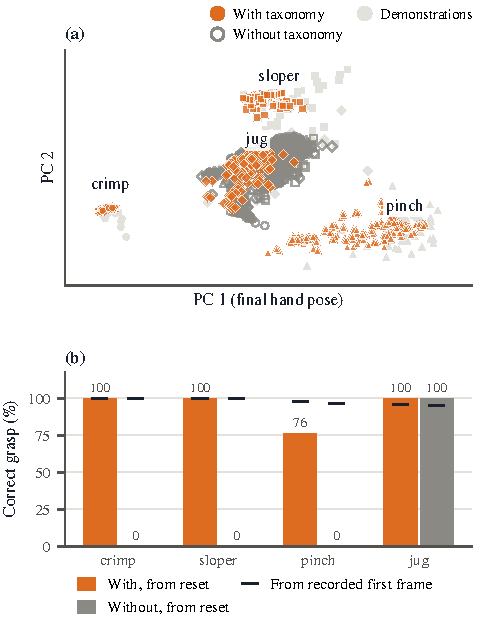
\includegraphics[width=\columnwidth]{fig_grasp_selection.pdf}
\caption{Which grasp each policy executes ($K=8$ closed-loop rollouts per input
$\times$ 25 inputs per grasp type, spring-testbed checkpoints). (a) Final hand poses
of rollouts started from the deployment reset pose, projected onto the first two
principal components of the demonstrators' final hand poses (light markers; marker
shape = grasp type of the hold). With taxonomy (filled), rollouts land on the
demonstrated grasp for their hold; without taxonomy (outlined), rollouts for every
hold land on the jug grasp. (b) Share of rollouts whose final hand pose is nearest the
correct grasp type. Bars: started from the reset pose; ticks: started from the first
frame of a recorded demonstration, where both policies are near 100\%.}
\label{fig:mech}
\end{figure}

\paragraph*{Latent-space separation}
We compute silhouette score and stratified 5-fold kNN accuracy on the fused encoder
output for the without-taxonomy policy using held-out inputs spanning all four grasp
types. Despite receiving no conditioning signal, the encoder reaches kNN accuracy
99\% and silhouette 0.32. The point-cloud branch alone does not separate the types
(silhouette $-0.03$, 5-NN accuracy 39\%, chance 25\%); all of this structure comes
from the proprioception channel (supplementary material).

\paragraph*{Mean action commitment}
We compute the between-type spread of mean predicted final-step hand poses across all
four grasp types. The without-taxonomy policy produces means that differ across
types at 90\% of the demonstrator's between-type spread (0.316\,rad vs.\ 0.352\,rad
for demonstrators; the with-taxonomy policy produces 0.314\,rad). From recorded
demonstration frames, the without-taxonomy
policy does not collapse to a single behavior mode.

\paragraph*{Closed-loop rollouts from the reset pose}
Both analyses above use the first frame of recorded demonstrations as input. At
deployment, every trial instead starts from one fixed reset pose. We therefore roll
out each policy in closed loop from that reset pose, replicating the evaluation loop
(200 steps at 10\,Hz, 8 of 16 predicted actions executed per replan, the hold's
recorded point cloud held fixed, commanded joints assumed tracked exactly), and assign
each final hand pose to the nearest demonstrator grasp-type mean (demonstrations
assign to their own type 99\% of the time). From the recorded first frame, both
policies execute the correct grasp in 98\% of rollouts. From the reset pose, the
with-taxonomy policy does so in 94\% (crimp, sloper, jug 100\%; pinch 76\%, with the
misses landing on jug), while the without-taxonomy policy does so in only 25\%: every
one of its 800 rollouts ends in a jug grasp, whatever the hold (Fig.~\ref{fig:mech}).

\paragraph*{Interpretation: taxonomy as a mode selector}
These results support the mode-selector account at deployment. During data
collection the operator positions the arm and hand under VR teleoperation before
recording begins, so the first recorded frame already holds a hand pre-shaped for its
grasp type (0.8--3.0\,rad from the reset pose) \todo{author: confirm hand was
pre-shaped at recording start}. The without-taxonomy policy learns to read grasp type from
this hand pose, which is why its latent separation comes from proprioception rather
than the point cloud. At deployment every trial starts from the same reset pose, that
cue is gone, and the point cloud cannot replace it because the encoder does not
separate the holds, so the policy defaults to a single grasp. The taxonomy label fills
in this missing information, acting as a switch that decides which grasp the policy
performs.

\subsection{Hardware Evaluation}
\label{sec:robot_eval}
We ran 80 paired trials = 160 rollouts (4 paired trials per orientation $\times$ 5
orientations $\times$ 4 hold types) in a single $\sim$7-hour session with a single
operator. No trial pegged the ratchet at $n = 11$, so the dataset is free of
right-censoring. Statistical tests are Wilcoxon signed-rank (two-sided) per grasp
type with $n=20$ pairs each; effect sizes are Cohen's $d$ on paired differences.

\begin{figure*}[t]
\centering
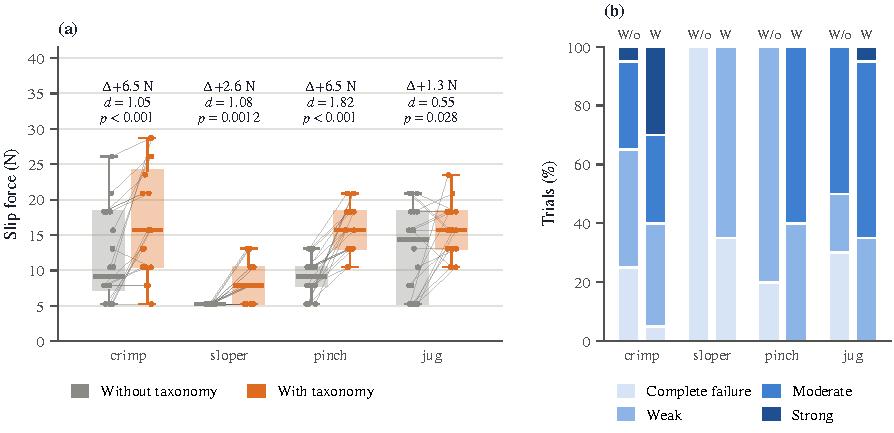
\includegraphics[width=\textwidth]{fig_hardware.pdf}
\caption{Hardware evaluation on the spring testbed (20 paired trials per grasp type,
80 total). (a) Per-trial slip force with vs.\ without taxonomy conditioning; boxes are
IQR with medians, thin lines join the two trials of each pair, and each type is
annotated with its median gain, Cohen's $d$ on paired differences, and Wilcoxon
signed-rank $p$ (two-sided). The without-taxonomy sloper box is degenerate (all 20
trials at preload force $\approx 5.2$\,N), a complete failure that conditioning
partly rescues. (b) Failure-mode breakdown (W = with taxonomy, W/o = without): each bar
stacks 20 trials into four force regimes. Conditioning converts 13 of the 20 complete
sloper failures into weak grips (7 remain at preload), and pinch and jug show no
complete failures with conditioning; crimp under
conditioning shows 6/20 strong grips versus 1/20 without.}
\label{fig:hw}
\end{figure*}

\paragraph*{H1: median slip force}
Taxonomy conditioning improves grip strength on every grasp type tested
(Fig.~\ref{fig:hw}a). Overall median slip force rises from 7.9\,N to
13.1\,N, a $+5.2$\,N (66\%) improvement (Wilcoxon $p < 0.001$,
Cohen's $d = 0.95$).

\paragraph*{H2: ordering across grasp types}
The effect-size ordering matches H2. Pinch, the narrowest hold, shows the largest
effect ($d = 1.82$), with the conditioned model winning all 20 pairs. Sloper
($d = 1.08$) and crimp ($d = 1.05$) follow. The jug gives the smallest effect
($d = 0.55$); it is the grasp the without-taxonomy policy defaults to, so on the jug
hold both policies usually perform the right grasp. Pinch and crimp share the same $\Delta$ median but
pinch's larger $d$ reflects a tighter distribution of paired differences. Aggregating
across types, the conditioned model wins 61 of 80 pairs, ties 14, and loses 5.

\paragraph*{Failure-mode rescue}
Bucketing each rollout into complete failure ($\le 5.3$\,N, preload only), weak grip
($5.3$--$13.5$\,N), moderate grip ($13.5$--$23.0$\,N), or strong grip ($> 23.0$\,N)
shows where the gain comes from. The bin boundaries correspond to
0, 1--3, 4--7, and $\ge 8$ ratchet teeth, respectively. Complete failures fall from 44\% of
trials without conditioning to 10\% with it (a $4.4\times$ reduction), and strong
grips rise from 1\% to 9\%. Most of the improvement comes from converting failed
trials into measurable grips, with smaller gains in the upper tail
(Fig.~\ref{fig:hw}b).

\paragraph*{Orientation profile}
Per-orientation breakdown shows the expected geometric pattern: performance peaks
near $0^\circ$ (pull-aligned) and degrades as the hold rotates toward $\pm 45^\circ$,
where the moment arm between contact and pull axis maximizes mechanical disadvantage
against the grip. Crimp shows the largest orientation sensitivity (18\,N spread
between hardest and easiest orientation), consistent with the thin lateral profile of
the crimp edge providing little angular tolerance (supplementary material).

\paragraph*{Methodological controls}
Strict global order alternation made each model run first in exactly 40 of 80 pairs.
A Mann--Whitney $U$ test between when-first and when-second rollouts found no
detectable order bias for either model (with $p = 0.771$, without $p = 0.690$). The
median between-trial PC centroid drift was sub-millimeter, well below the post-hoc
15\,mm drift filter threshold, and no pairs were dropped.

% -----------------------------------------------------------------------
\section{Discussion}
\label{sec:discussion}
% -----------------------------------------------------------------------

\paragraph*{Failure-mode rescue as the dominant mechanism}
The gain from conditioning is concentrated in the lower tail of the slip-force
distribution. This follows from the mode-selector result: without the label,
the policy executes a jug grasp on crimp, sloper, and pinch holds, and a grasp shaped
for the wrong hold slips under load.

\paragraph*{Why climbing holds}
Each climbing hold needs its own grasp, but the policy's point-cloud encoder can't tell
the holds apart. Without the label, the policy has nothing reliable to pick the grasp
from at deployment, and the taxonomy label gives it that. We expect the same to be true
for other objects that look alike to a 3D encoder but need different hand shapes.

\paragraph*{Benchmark design}
The spring displacement testbed provides experimental control unavailable in standard
pick-and-place lift tests: the pull direction and magnitude are fixed by hardware,
and the ratchet gives a continuous reading rather than a threshold-dependent binary.

\paragraph*{Limitations}
All 200 training episodes come from one operator and one teleop session, and each
grasp category is represented by exactly one physical hold. The per-type effect sizes
reported here therefore conflate ``the conditioning effect on that grasp
type'' with ``the conditioning effect on this hold.'' A held-out crimp variant
(\textit{test\_edge}) is collected but not evaluated in this paper. The specific
Cohen's $d$ values are platform-specific (Franka + LEAP only) until shown otherwise.
The spring testbed measures grip force against displacement on one fixed axis, which
captures the dominant load direction of dynamic crux moves but not multi-directional
or sustained loads. Training did not pin a global random seed, and the planned
wrong-label ablation, where the conditioned policy is given a deliberately wrong label
to test causality, has not been run yet. The closed-loop rollouts in
\S\ref{sec:mechanistic} are simulated (commanded joints tracked exactly, no contact),
and the grasp each policy executed was not logged on hardware. We also cannot yet
separate two explanations for the point-cloud result: the holds' point clouds may be
too similar after cropping and downsampling, or the policy may have relied on the
hand-pose cue during training instead of learning from the scan. All 80 paired trials come from one $\sim$7-hour
session with one rater, so inter-session variance is uncharacterized. Hold orientation
is not stored in the training zarr; the policy infers it from the point cloud. Finally,
median slip force with conditioning is 13.1\,N, which is a moderate grip, so there is
still room to improve with per-grasp specialization or more data.

% -----------------------------------------------------------------------
\section{Conclusion}
% -----------------------------------------------------------------------
We presented BetaGrasp, a grasp-taxonomy-aware 3D diffusion policy for dexterous
climbing hold manipulation, together with a climbing-hold benchmark on a
spring-constrained displacement testbed instrumented with a linear ratchet that
yields a continuous slip-force readout. Our main finding is that taxonomy conditioning
acts as a \textbf{mode selector}, or switch, for which grasp the policy performs. The without-taxonomy policy separates grasp types only when its
starting hand pose already encodes them, since its point-cloud encoder does not tell
the holds apart; from the deployment reset pose it collapses to
a single jug grasp, while the conditioned policy selects the correct grasp in 94\% of
rollouts. Hardware evaluation on 80 paired trials supports this
account: median slip force rises by 5.2\,N with conditioning, the smallest effect is
on the jug, the grasp the without-taxonomy policy defaults to, and the complete-failure
rate falls from 44\% of trials to 10\%.

\paragraph*{Reproducibility}
The two checkpoints (with and without taxonomy) are a matched ablation pair, identical
except for the grasp-type encoder branch (\S\ref{sec:arch}). All figures in this paper
regenerate from the released evaluation JSON via the included analysis scripts. Code,
training data, and checkpoints will be released \todo{anonymized links}; CAD, 3D-print
files, and a parts list for the spring testbed will be released on acceptance.

\bibliographystyle{IEEEtran}
\bibliography{references}

\end{document}
